\part*{ابزارهایی برای استفاده در سندباکس}
\chapter{استفاده از اوراکل
    \lr{«MySql Workbrench»}
    }
یاین ابزار گرافیکی برای مدیریت بانک‌های اطلاعاتی مای‌اس‌کیوال در اکثر سیستم‌عامل‌ها قابل نصب است. برای استفاده از آن کافی است این برنامه را در سیستم‌عامل  یا توزیع سیستم میزبان و سیستم مورد استفاده خود نصب کنید. سپس با استفاده از دکمه دارای نقشک به‌علاوه «+» کنار عبارت اتصال‌های من 

\lr{«My Connections»}
،
 اتصال جدیدی را ایجاد نمایید. در هنگام کلیک بر روی این دکمه، پنجره مشابه پنجره زیر نمایش داده خواهد شد که با پر کردن مقادیر به صورت مناسب می‌توانید به مای‌اس‌کیوال موجود در سندباکس دست یابید.  برای نوشتن گذرواژه باید روی دکمه 
\lr{ «Store in keychains»} 
 کلیک کنید. \ref{Oracle-MWB}
\begin{figure}
    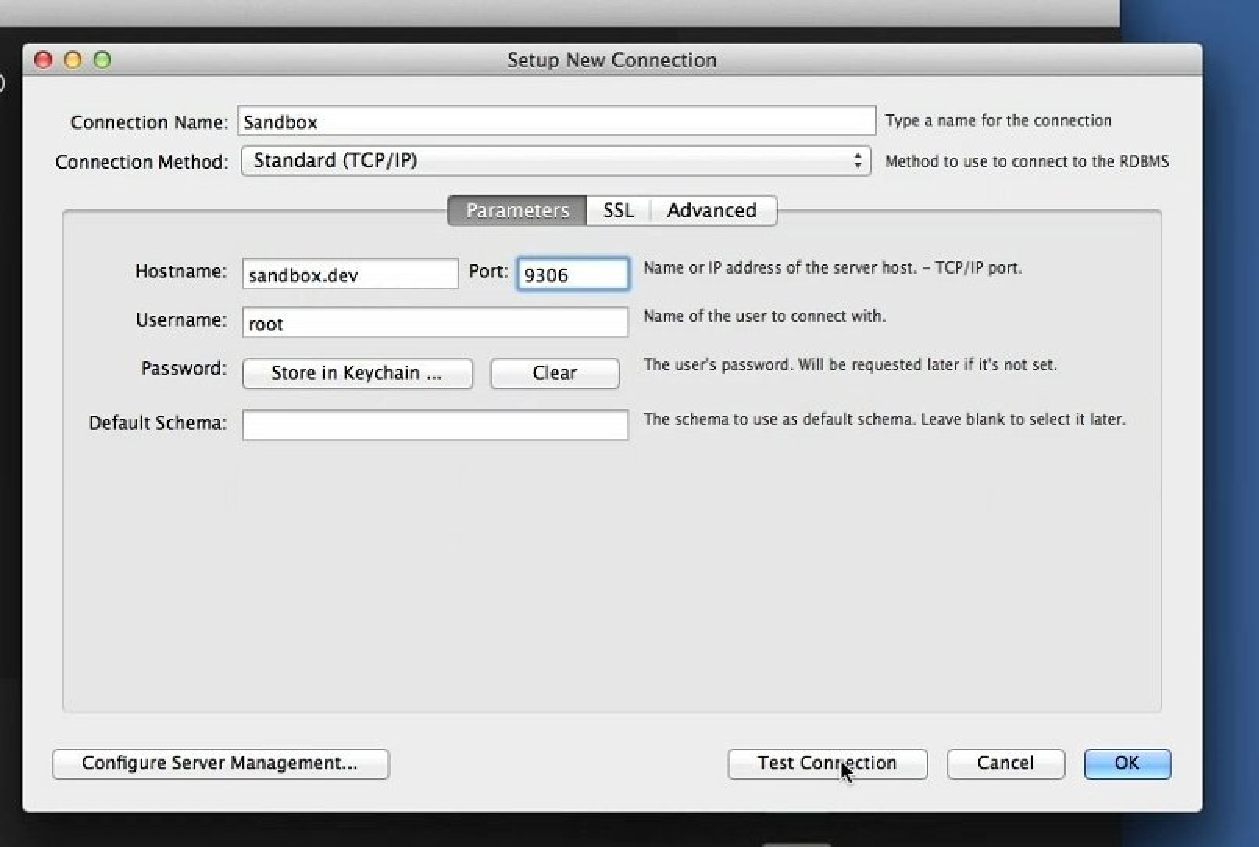
\includegraphics[width=.9\textwidth ,height=.65\textwidth]{Pic/MWB}
    \caption{ اتصال از  طریق نرم افزار 
     \lr{MySQL Workbrench}   
        }
    \label{Oracle-MWB}
\end{figure}

بعد از آن اگر بر دکمه 
\lr{«Test Connection»}
 کلیک کنید، برقراری ارتباط بررسی می‌شود که در صورت پیغام درستی ارتباط می‌توانید بر دکمه OK کلیک کنید. حال با کلیک مضاعف (دو‌بارکلیک) بر روی کادر ایجاد شده در نرم‌افزار، می‌توانید وارد صفحه مربوط به ارتباط شوید که شامل اطلاعاتی اولیه از ویرایش اوبونتو و مای‌اس‌کیوال نمایش داده شده است. البته در ابتدا کادری جهت نوشتن فرامین اس‌کیوال مشاهده می‌شود که اگر از سمت چپ برنامه، بر پیوند وضعیت سرور 
 \lr{«Server-Status»}
  کلیک کنید، اطلاعات دیگری مانند اطلاعات و جزئیات سرور و … نیز از این طریق قابل مشاهده اند. \ref{Oracle-MWB-UI}
\begin{figure}
    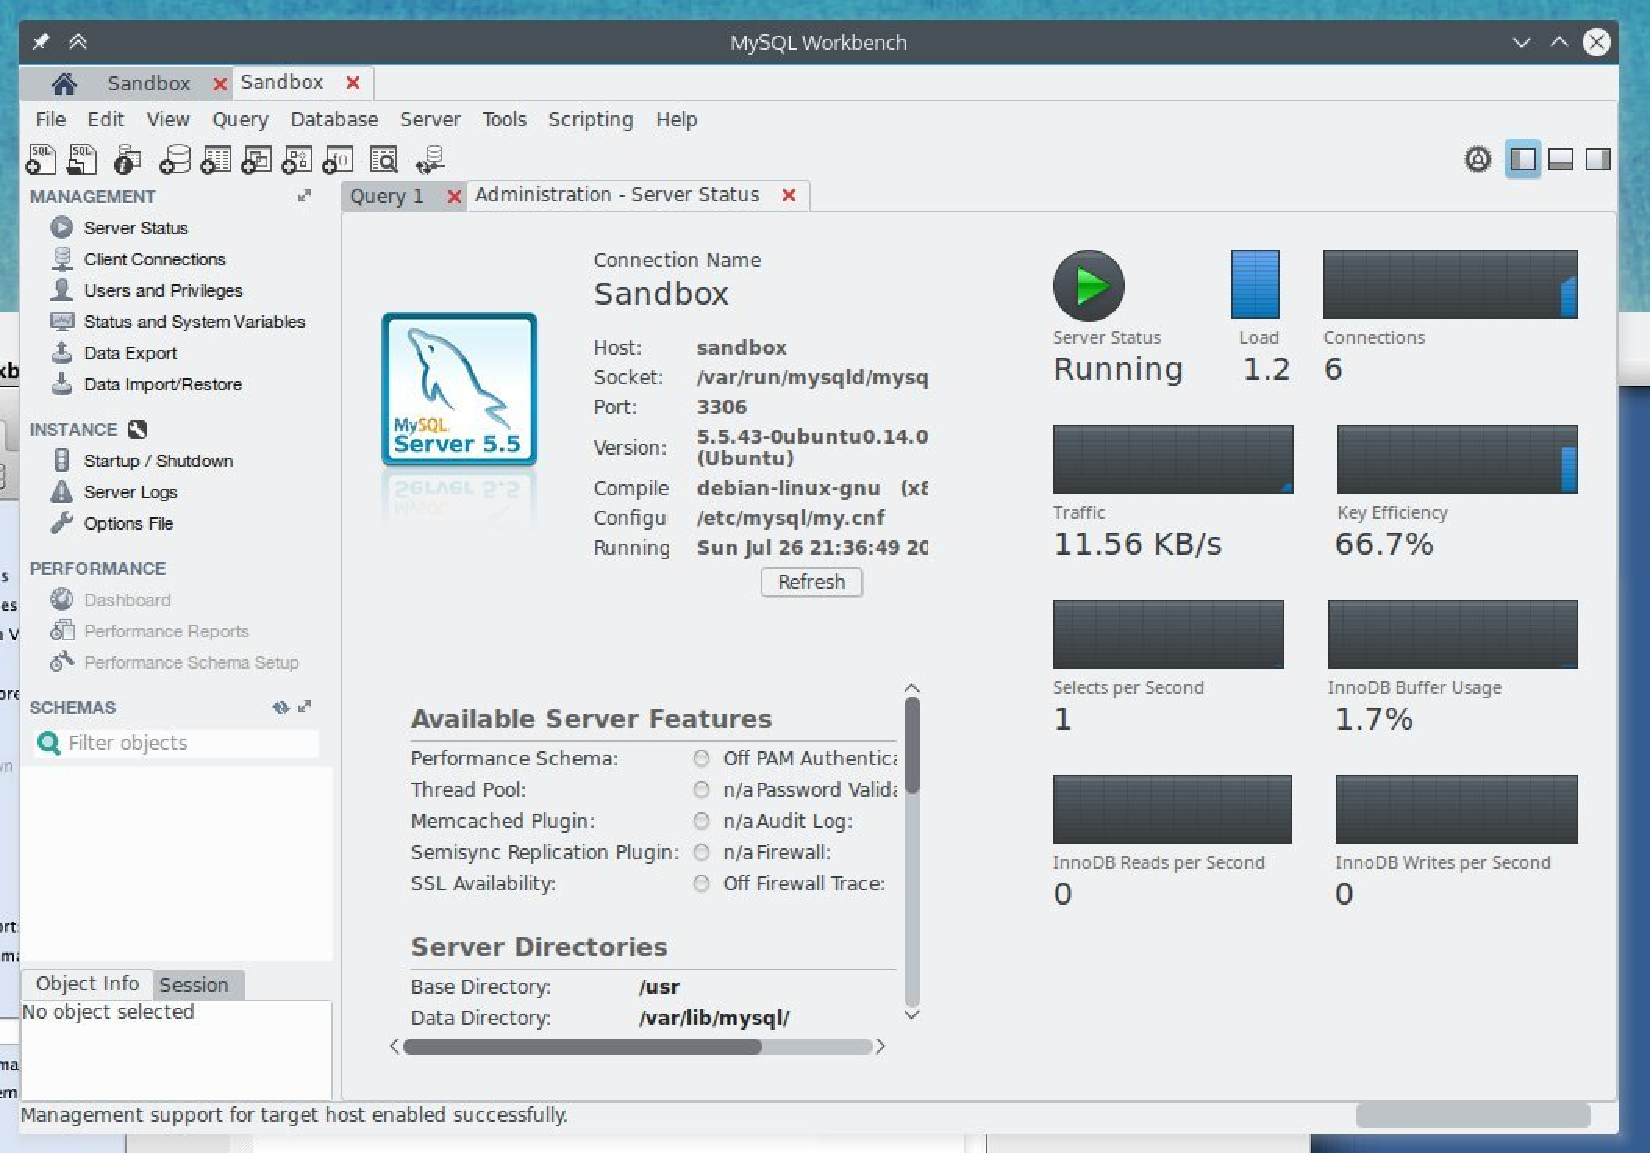
\includegraphics[width=.9\textwidth ,height=.65\textwidth]{Pic/MWB2}
    \caption{ نمایی از نرم افزار 
        \lr{MySQL Workbrench}   
    }
    \label{Oracle-MWB-UI}
\end{figure}